\documentclass[12pt,letterpaper]{article}

\usepackage[utf8]{inputenc}
\usepackage[letterpaper,margin=1in]{geometry}
\usepackage{caption} % for table captions

\usepackage{amsmath} % for multi-line equations and piecewises
\usepackage{indentfirst} % to indent after a section
\usepackage{setspace}
\usepackage{times}
\usepackage{graphicx}
\usepackage{textcomp}
\usepackage{xspace}
\usepackage{verbatim} % for block comments
\usepackage{subfig} % for subfigures
\usepackage{enumitem} % for a) b) c) lists
\usepackage{float}
\newcommand{\Cyclus}{\textsc{Cyclus}\xspace}%
\usepackage{titling}
\newcommand{\subtitle}[1]{%
  \posttitle{%
    \par\end{center}
    \begin{center}\large#1\end{center}
    \vskip0.5em}%
}
\usepackage{tikz}


\usetikzlibrary{shapes.geometric,arrows}
\tikzstyle{process} = [rectangle, rounded corners, minimum width=3cm, minimum height=1cm,text centered, draw=black, fill=blue!30]
\tikzstyle{arrow} = [thick,->,>=stealth]


\graphicspath{{images/}}
 
\usepackage[font={footnotesize,it}]{caption}
 



\setlength{\parindent}{15pt} % Default is 15pt.




\fontfamily{ptm}\selectfont

\title{Numerical Experiments for Validating Prediction Algorithms Report}
\subtitle{Draft 1}
\author{Jin Whan Bae and Gwendolyn Chee}
\date{2017-09-23}


\begin{document}
	
	\maketitle
	\hrule
	\onehalfspacing
	\thispagestyle{empty}

\section*{Introduction}
The Demand-Driven Cycamore Archetype project (NEUP-FY16-10512) aims to develop \Cyclus in-situ demand-driven deployment capabilities through non-optimizing, deterministic-optimizing and stochastic-optimizing prediction algorithms.

These prediction models are being developed by the University of South Carolina. In this report, we discuss numerical experiments for testing the non-optimizing, deterministic and stochastic optimizing methods. 

\section{Once through Nuclear Fuel Cycle}
This section evaluates the required tests for
each method assuming a once-through fuel cycle.

\begin{figure}[H]
\caption{Flow Chart of Once through Nuclear Fuel Cycle}
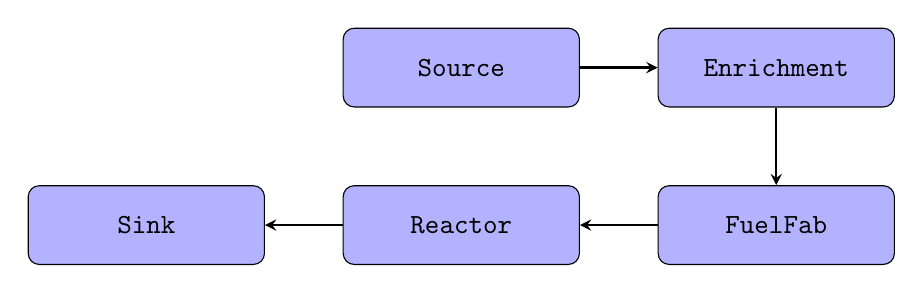
\begin{tikzpicture}[node distance=2cm]
\node (source) [process] {\texttt{Source}};
\node (enrichment) [process, right of=source, xshift=2cm] {\texttt{Enrichment}};
\node (fuelfab) [process, below of=enrichment] {\texttt{FuelFab}};
\node (reactor) [process, left of=fuelfab, xshift = -2cm]{\texttt{Reactor}};
\node (sink) [process, left of=reactor, xshift = -2cm]{\texttt{Sink}};

\draw [arrow] (source) -- (enrichment); 
\draw [arrow] (enrichment) -- (fuelfab); 
\draw [arrow] (fuelfab) -- (reactor);
\draw [arrow] (reactor) -- (sink);
\end{tikzpicture}
\end{figure}

\subsection*{Non-optimizing prediction method}
Conditions for test to satisfy: 
\begin{itemize}
\item  Do all the reactors run at full capacity (not lacking fuel)? 
\item Is the input required by the reactors within a specific uncertainty of the analytic solution? 
\item  Is the output of the fuel fabrication facilities within a specific range (more than?) of the input required by the reactors (calculated by the analytic solution) for all of them to run for each time step? 
\begin{itemize}
\item Is a new fuel fabrication facility deployed when the input required by the reactors exceeds the output of current fuel fabrication facilities?
\item Is a fuel fabrication facility decommissioned when the input required by the reactors falls behind the output of current fuel fabrication facilities?
\end{itemize}
\item  Is the output of the enrichment facilities within a specific range of the input required by the fuel fabrication facilities (calculated by the analytic solution) for each time step? 
\begin{itemize}
\item Is a new enrichment facility deployed when the input required by the fuel fabrication facilities exceeds the output of current enrichment facilities?
\item Is a enrichment facility decommissioned when the input required by the fuel fabrication facilities falls behind the output of current enrichment facilities?
\end{itemize}
\item Is the output of the conversion facilities within a specific range of the input required by the enrichment facilities (calculated by the analytic solution) for each time step? 
\begin{itemize}
\item Is a new conversion facility deployed when the input required by the enrichment facility exceeds the output of current conversion facilities?
\item Is a conversion facility decommissioned when the input required by the enrichment facilities falls behind the output of current conversion facilities?
\end{itemize}
\item Is the output of the milling facilities within a specific range of the input required by the conversion facilities (calculated by the analytic solution) for each time step? 
\begin{itemize}
\item Is a new milling facility deployed when the input required by the conversion facility exceeds the output of current milling facilities?
\item Is a milling facility decommissioned when the input required by the conversion facilities falls behind the output of current milling facilities?
\end{itemize}
\item Is the output of uranium mining within a specific range of the input required by the milling facilities (calculated by the analytic solution) for each time step? 
\begin{itemize}
\item Does the amount of uranium mined increase when the input required by the milling facility exceeds the output of current uranium mines?
\item Does the amount of uranium mined decrease when the input required by the milling facilities falls behind the output of current uranium mines?
\end{itemize}
\end{itemize}

\subsection*{Deterministic-Optimizing/Stochastic prediction method}
Conditions for test to satisfy: 
\begin{itemize}
\item 
\end{itemize}


\section{Advanced Fuel Cycles}
Advanced fuel cycles denote the fuel cycles
where reprocessing of spent fuel takes place,
to create fuel for advanced reactors. 
\end{document}






